

\subsection{\textit{Graphical Representation}}

	\textit{To effectively demonstrate visually, on what the transforms and the series means and what it does to functions, we shall specifically consider the function $f(t) = e^{-t}\cdot\sin\left(2t\right)$, as this function contains both an exponential component and a sinusoidal component.}

	\subsubsection{\textit{The Laplace Transform}}

		\textit{}

			\begin{figure}[H]
			\centering
			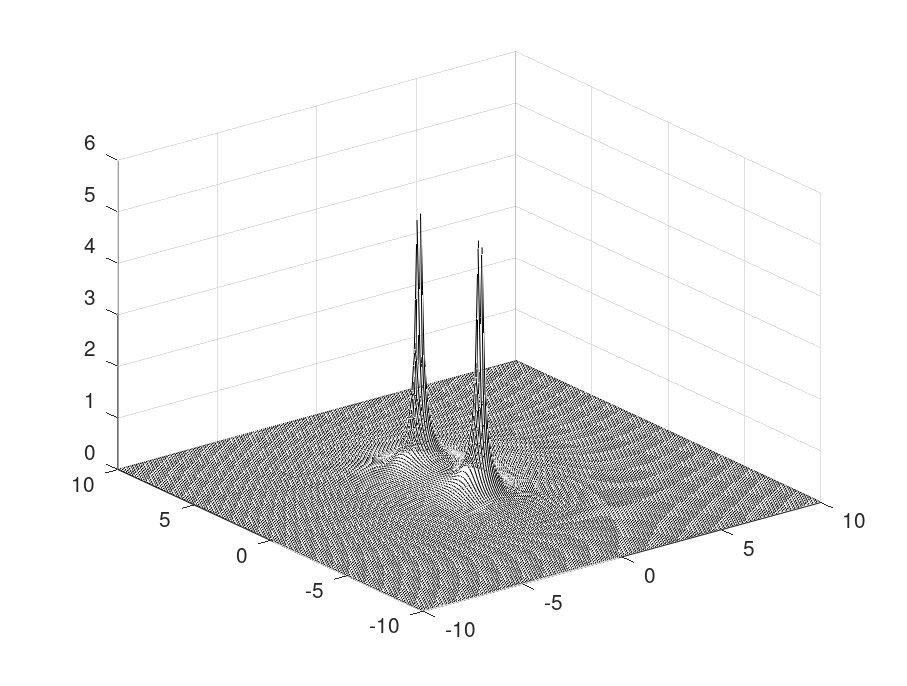
\includegraphics[width=15cm]{LapPictures/bk.png}
    			\caption{\textit{The Laplace transform of $e^{-x}\cdot\sin\left(2x\right)$}}
			\end{figure}

	\subsubsection{\textit{The Fourier Transform}}

		\textit{}

			\begin{figure}[H]
			\centering
			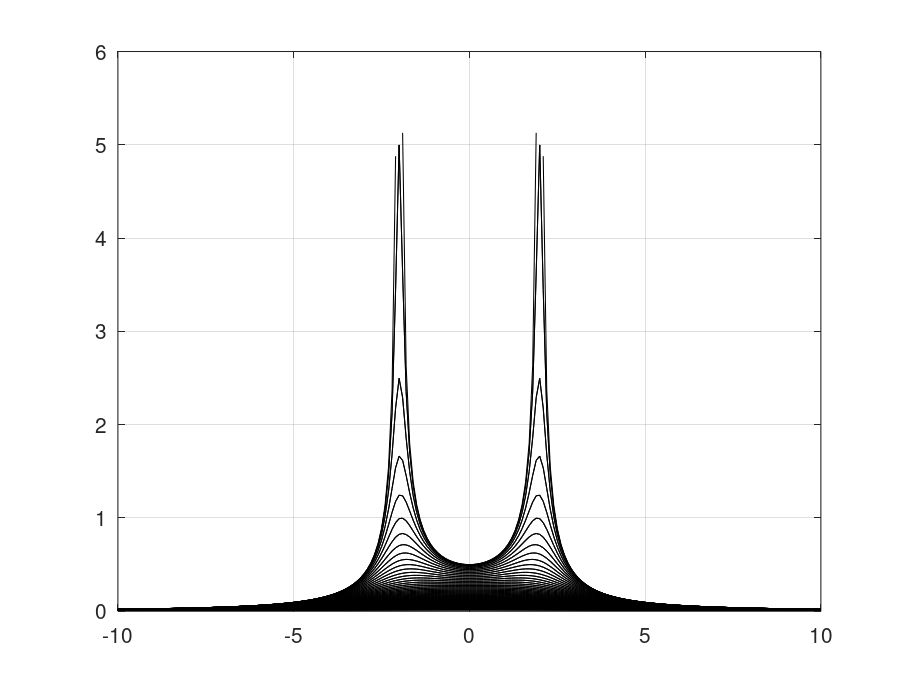
\includegraphics[width=15cm]{FouPictures/bk.png}
    			\caption{\textit{The Fourier transform of $e^{-x}\cdot\sin\left(2x\right)$}}
			\end{figure}

	\subsubsection{\textit{The Fourier Series}}

		\textit{}

			\begin{figure}[H]
			\centering
			\includegraphics[width=15cm]{}
    			\caption{\textit{The Fourier series of $e^{-x}\cdot\sin\left(2x\right)$}}
			\end{figure}


